\documentclass[tikz, border=15pt]{standalone}
\usepackage{amsmath}
\usetikzlibrary{positioning, arrows.meta, shapes.geometric, calc, backgrounds, fit}

% Color definitions
\definecolor{navyblue}{HTML}{2c5282}
\definecolor{appgreen}{HTML}{38a169}
\definecolor{resgold}{HTML}{d69e2e}

\begin{document}
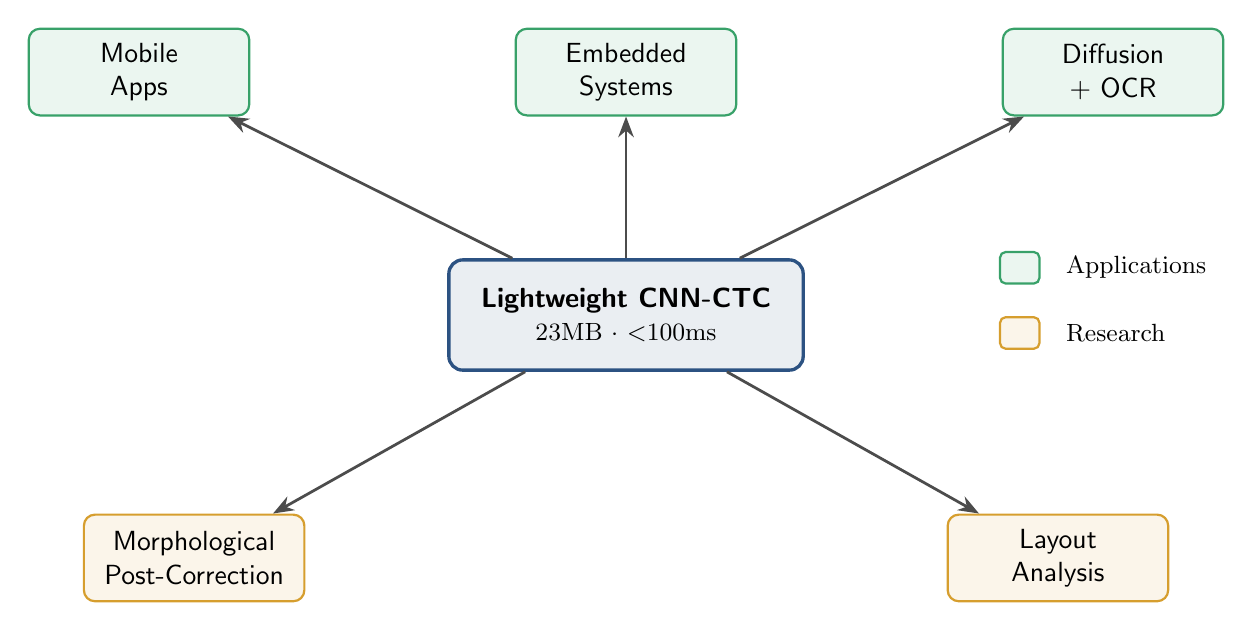
\begin{tikzpicture}[
    font=\sffamily,
    >=Stealth,
    node distance=1.5cm and 1.2cm,
    % Central model node
    central/.style={
        draw=navyblue, thick, line width=1.2pt,
        rectangle, rounded corners=5pt,
        minimum width=4.5cm, minimum height=1.4cm,
        align=center, fill=navyblue!10,
        font=\sffamily\bfseries
    },
    % Application nodes (green)
    app/.style={
        draw=appgreen, thick,
        rectangle, rounded corners=4pt,
        minimum width=2.8cm, minimum height=1.1cm,
        align=center, fill=appgreen!10
    },
    % Research nodes (gold)
    research/.style={
        draw=resgold, thick,
        rectangle, rounded corners=4pt,
        minimum width=2.8cm, minimum height=1.1cm,
        align=center, fill=resgold!10
    },
    % Arrow style
    arrow/.style={->, thick, draw=black!70, line width=1pt},
    % Legend style
    legendbox/.style={
        draw=black!50, thick,
        rectangle, rounded corners=2pt,
        minimum width=0.5cm, minimum height=0.4cm,
        inner sep=2pt
    }
]

% Central node
\node[central] (cnn) {Lightweight CNN-CTC\\{\normalfont\small 23MB $\cdot$ $<$100ms}};

% Application nodes (top row)
\node[app, above left=1.8cm and 2.5cm of cnn] (mobile) {Mobile\\Apps};
\node[app, above=1.8cm of cnn] (embedded) {Embedded\\Systems};
\node[app, above right=1.8cm and 2.5cm of cnn] (diffusion) {Diffusion\\+ OCR};

% Research nodes (bottom row)
\node[research, below left=1.8cm and 1.8cm of cnn] (morpho) {Morphological\\Post-Correction};
\node[research, below right=1.8cm and 1.8cm of cnn] (layout) {Layout\\Analysis};

% Arrows from central to applications
\draw[arrow] (cnn) -- (mobile);
\draw[arrow] (cnn) -- (embedded);
\draw[arrow] (cnn) -- (diffusion);

% Arrows from central to research
\draw[arrow] (cnn) -- (morpho);
\draw[arrow] (cnn) -- (layout);

% Legend (positioned far bottom-right, outside diagram)
\begin{scope}[shift={(5.0, 0.6)}]
    \node[legendbox, fill=appgreen!10, draw=appgreen] (leg1) {};
    \node[right=0.2cm of leg1, font=\small] {Applications};
    \node[legendbox, fill=resgold!10, draw=resgold, below=0.4cm of leg1] (leg2) {};
    \node[right=0.2cm of leg2, font=\small] {Research};
\end{scope}

\end{tikzpicture}
\end{document}
